\documentclass[manuscript,screen]{article}
\usepackage{tikz}
\usepackage{amsmath,amsthm}
\usetikzlibrary{positioning,automata,fit,shapes,calc}
\usepackage{pgfplots}
\pgfplotsset{width=10cm,compat=1.9}
\usepackage{amssymb}
\usepackage{tikz}

\newcommand{\goal}{\mathit{goal}}

\newcommand{\fail}{\mathit{fail}}

\newcommand{\wgt}{\mathit{wgt}}

\begin{document}

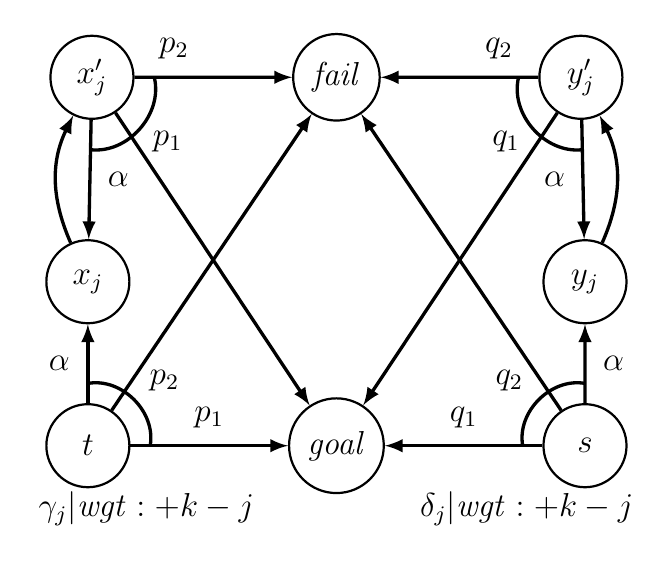
\begin{tikzpicture}[scale=.9,auto,node distance=8mm,>=latex]
\large
    \tikzstyle{round}=[thick,draw=black,circle]
    
   
    \node[round,minimum size=30pt] (t) {$t$};
    \node[round,above=10mm of t, minimum size=30pt] (xj) {$x_j$};
 

    
    \node[round, right=20mm of t ,minimum size=30pt] (goal) {$\goal$};
     \node[round, right=20mm of goal ,minimum size=30pt] (s) {$s$};
     \node[round,above=10mm of s, minimum size=30pt] (yj) {$y_j$};

    

    \node[round,above=35mm of goal, minimum size=30pt] (fail2) {$\fail$};
    \node[round,left=20mm of fail2, minimum size=30pt] (xj2) {$x_j^\prime$};
    \node[round,right=20mm of fail2, minimum size=30pt] (yj2) {$y_j^\prime$};


    
    
    
    
%%%%% Initial component
  \draw[color=black , very thick,->] (t) edge   node [pos=0.10,right=2pt] {$p_2$} (fail2) ;
  \draw[color=black , very thick,->] (t)  edge node [very near start, anchor=center] (h2) {} node [pos=0.5,above=2pt] {$p_1$} node [pos=0.1,below=12pt] {$\gamma_j|\wgt:+k-j$} (goal) ;
   \draw[color=black , very thick, ->] (t) edge node [ near start, anchor=center] (h1) {} node [pos=0.5,left=2pt] {$\alpha$} (xj);
  \draw[color=black , very thick] (h1.center) edge [bend left=55] node [pos=0.25,above=2pt] {} (h2.center);
  
   \draw[color=black , very thick,->] (xj2) edge  node [very near start, anchor=center] (g2) {}  node [pos=0.25,above=2pt] {$p_2$} (fail2) ;
  \draw[color=black , very thick,->] (xj2)  edge node [pos=0.1,right=2pt] {$p_1$} (goal) ;
   \draw[color=black , very thick, ->] (xj2) edge node [ near start, anchor=center] (g1) {} node [pos=0.5,right=2pt] {$\alpha$} (xj);
  \draw[color=black , very thick] (g2.center) edge [bend left=55] node [pos=0.25,above=2pt] {} (g1.center);
  
  \draw[color=black , very thick, ->] (xj) edge [bend left=25] (xj2);

  
      \draw[color=black , very thick,->] (s) edge   node [pos=0.10,left=2pt] {$q_2$} (fail2) ;
  \draw[color=black , very thick,->] (s)  edge node [very near start, anchor=center] (j1) {} node [pos=0.5,above=2pt] {$q_1$}node [pos=0.1,below=12pt] {$\delta_j|\wgt:+k-j$} (goal) ;
   \draw[color=black , very thick, ->] (s) edge node [ near start, anchor=center] (j2) {} node [pos=0.5,right=2pt] {$\alpha$}  (yj);
  \draw[color=black , very thick] (j1.center) edge [bend left=55] node [pos=0.25,above=2pt] {} (j2.center);
  
   \draw[color=black , very thick,->] (yj2) edge  node [very near start, anchor=center] (k2) {}  node [pos=0.25,above=2pt] {$q_2$} (fail2) ;
  \draw[color=black , very thick,->] (yj2)  edge node [pos=0.1,left=2pt] {$q_1$} (goal) ;
   \draw[color=black , very thick, ->] (yj2) edge node [ near start, anchor=center] (k1) {} node [pos=0.5,left=2pt] {$\alpha$} (yj);
  \draw[color=black , very thick] (k1.center) edge [bend left=55] node [pos=0.25,above=2pt] {} (k2.center);
  
  \draw[color=black , very thick, ->] (yj) edge [bend right=25] (yj2);
    
\end{tikzpicture}

\end{document}